\subsection{Needle variations}
In the beginning of section 3 we talked about the variations of trajectories, and analyzed those variations \textit{a-posteriori}, trying to describe them. Now we are going to see, so to say, \textit{the elementary (infinitesimal) way of producing said variations.} This will be of course through control variations, not through the variation of initial condition.


\paragraph{Needle variation (fixed interval)}
et \controlSystem be a control system, $x_0\in\chi$ be an initial condition for eq. \ref{e1.1}, $\tzto\subset\R$ a time interval, $\mu\in\admContr{x_0,t_0,\tzto}$. We then define 
\lista{
	\item \grass{fixed interval needle variation \underline{data}} as a triple $\theta=(\tau_\theta,l_\theta,\omega_\theta)$ for which \lista{
		\item $\tau_\theta\in(t_0,t_1]$
		\item $l_\theta\in\R_{\geq0}$
		\item $\omega_\theta\in U$
	}

	\item the \grass{control variation} of the control $\mu$ associated to the relative fixed interval needle variation data $\theta$ is the map $\mu_\theta$ is the map $mu_\theta:J\times\tzto\fd U$ such that
	\[\mu_\theta = \left\{ \begin{array}{lr}
	\omega_\theta & \mbox{if $t\in[\tau_\theta-s*l_\theta,\tau_\theta]$}\\
	\mut & \mbox{otherwise}.\end{array}
	\right.	\]
	Where $J=[0,s_0]$ is an interval sufficiently small so that $\mu_\theta(s,t)$ is an admissible control for each $s\in J$
	Just to have an idea, this is how the function $\mu_\theta$ can look like for a certain $s>0$
	\begin{figure}[H]
		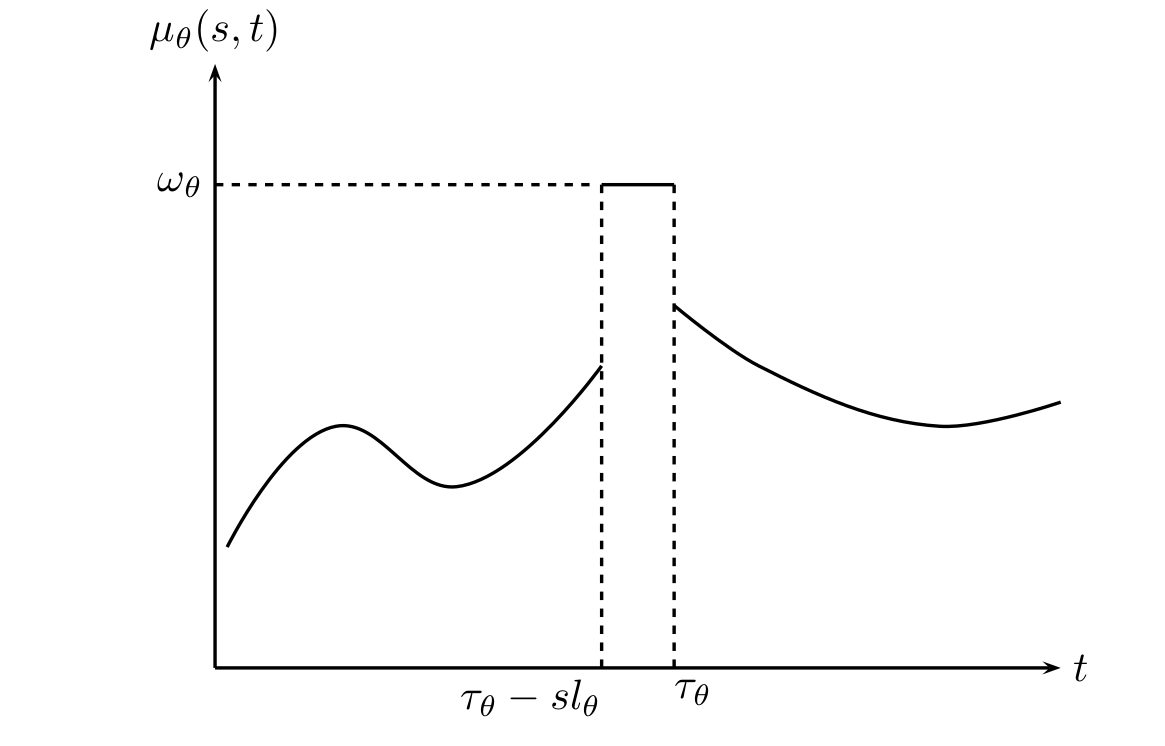
\includegraphics[width=\linewidth]{imgs/needle-variation.png}
		\caption{}
		\label{fig-needle-variation}
	\end{figure}
	\item \grass{fixed interval needle (\textit{infinitesimal})variation} associated with the control $\mu$, the trajectory \trajWinCond{\cdot} and the variation data $\theta$ as a vector of $\R^n$ defined as 
	\[v_\theta = \frac{d}{ds}\bigg|_{s=0} \xi(\mu_\theta(s,\cdot),x_0,t_0,\tau_\theta),\] when such derivative exists
}
This limit exists at almost any instant, since it exists for every instant that is a Lebesgue point for $t\fd f(\trajWinCondMath{t},\mut)$. Before stating this formally, we need the definition of $Leb(\mu,x_0,t_0,t)$: it's the set of Lebesgue points if $\tau\fd f(\trajWinCondMath{\tau},\mu(\tau)), \tau\in(t_0,t)$. Then,

\paragraph[prop 4.9]{Theorem:existence and form of fixed interval needle variations}\mbox{}\\
Let \controlSystem be a control system, $x_0\in\chi$ be an initial condition for eq. \ref{e1.1}, $\tzto\subset\R$ a time interval, $\mu\in\admContr{x_0,t_0,\tzto}$. Let then $\theta=(\tau_\theta,l_\theta,\omega_\theta)$ be a fixed interval needle variation data, with $\tau_\theta\in Leb(\mu,x_0,t_0,t_1)$. Then the fixed interval variation associated with those data exists and it's given by
\[ v_\theta=l_\theta*\bigg(f(\trajWinCondMath{\tau_\theta},\omega_\theta) - f(\trajWinCondMath{\tau_\theta},\mu(\tau_\theta) )  \bigg) \]

\subparagraph[4.10]{Variations and cones} The real importance of this theorem is not only in the fact that it is (almost) always possible to individuate the infinitesimal variation, but also in the fact that those variations form a cone, which is, if one vector represents a variation, then all of the half-line (originating from $0\in\R^n$) given by that vector is made up of fixed interval variations. Formally said, \\\\

\grass{Proposition:} Let \controlSystem be a control system, $x_0\in\chi$ be an initial condition for eq. \ref{e1.1}, $\tzto\subset\R$ a time interval, $\mu\in\admContr{x_0,t_0,\tzto}$. Let then \fivData be a fixed interval needle variation data, with $\tau_\theta\in Leb(\mu,x_0,t_0,t_1)$.\\
Then, the set of fixed interval needle variation associated with the data $\theta$ form a cone.\\\\
\grass{Proof:} It's just enough to say that, if $v_\theta$ is the variation associated with the data \fivData, then, taken a $k\in\R_{\geq0}, kv_\theta$ is the variation associated with the data $k\theta=(\tau_\theta,k*l_\theta,\omega_\theta)$. Using obvious notation, one could then say that $v_{k\theta}=kv_\theta$.\\\\
It is interesting to note that, in the triple representing the data, only the \textit{"lenght of the disturbance"} gets multiplied by the scalar. This means, that, referring to \ref{fig-needle-variation}, the final control is practically the same. In fact, the actual length of the horizontal step in the figure doesn't really matter, since s tends to zero, and the actual disturbance gets reduced to a (Lebesgue-neglettable) single point in time. \\
The only effect one may obtain is that, given a certain trajectory, the trajectories associated with varied control depart from the undisturbed one at a higher rate with growing s (at least, as long as s is small enough so that one can linearize the effect of control variation), but in the same direction. This is the same exact meaning of the length of the dotted arrows in \ref{fig-variations}.


\subsection{Multi-needle variations}
The concept behind multi needle variations is that they are made of single needle variations which sum up(linearly, as can be see in the relative theorem). We need this object basically because although single needle variations do form a cone, this is not generally convex. Convexity is needed in the proof, to find a hyperplane that separates the half space containing cone from another one. This is because a variational cone originating from the boundary of the reachable set cone will point toward the "less optimal", this half space is the non optimal one.\\\\
So now let \controlSystem be a control system, $x_0\in\chi$ be an initial condition for eq. \ref{e1.1}, $\tzto\subset\R$ a time interval, $\mu\in\admContr{x_0,t_0,\tzto}$. We want to define
 \lista{
	\item the \grass{fixed interval multi-needle variation data $\Theta$} as the collection $\Theta=\{\theta_1,..,\theta_k\}$ of fixed interval needle variation data $\theta_j=(\tau_j,l_j,\omega_j),j=1,..,k$, with the times $\tau_j$ all distinct.
	
	\item the \grass{control variation} of the control $\mu$ associated with the relative data $\Theta$ as the map $\mu_\Theta:J\times\tzto\fd U$ such that
	\[\mu_\Theta = \left\{ \begin{array}{ll}
	\omega_j & \mbox{if $t\in[\tau_\Theta-s*l_\Theta,\tau_\Theta],j=1,..,k$}\\
	\mut & \mbox{otherwise}.\end{array}
	\right.	\]
	Where $J=[0,s_0]$ is an interval sufficiently small so that $\mu_\Theta(s,t)$ is an admissible control for each $s\in J$.
	
	\item the \grass{fixed interval multi-needle variation} associated with the control $\mu$, the trajectory \trajWinCond{\cdot}, the time $t\in\tzto$ taken such that $t>\underset{j}{\max}(\tau_j)$ and the variation data $\Theta$ as a vector of $\R^n$ (a vectorial function of time actually) defined like this: 
	\[v_\theta(t) = \frac{d}{ds}\bigg|_{s=0} \xi(\mu_\Theta(s,\cdot),x_0,t_0,t),\] when such derivative exists
}

\paragraph[4.12]{Theorem: existence of multi-needle fixed interval variations}\mbox{}\\
Let \controlSystem be a control system, $x_0\in\chi$ be an initial condition for eq. \ref{e1.1}, $\tzto\subset\R$ a time interval, $\mu\in\admContr{x_0,t_0,\tzto}$. Then, let $\Theta=\{\theta_1,..,\theta_k\}$ be a multi needle variation data ("fixed interval" will from now on be omitted, since this case is the only one treated in this essay),$\Theta$ such that the times $\tau_j\in Leb(\mu,x_0,t_0,t)$, are all distinct, and also $t>\underset{j}{\max}(\tau_j)$.\\
Then, the multi needle variation is given by
\[v_\Theta(t)=\sum_{j=1}^{k}\fondMatMath{\tau_j}{t}\cdot v_{\theta_j} \]
As one can see, the variations caused by the various single needle variations first are let evolve in time from the instant in which they are applied to the "current" one, $t$, and then their effects sum up linearly.\\\\
Taking this into account, and also considering the fact that $v_{k\theta_j}=kv_{\theta_j}$ for whatever $k\geq0$ real, and remembering that the matrix-vector product is linear with respect to scalar multiplication, one can easily get the following
\subparagraph[4.13]{Corollary: coned convex combination of multi needle variations} With slight abuse of notation, given the usual control system, admissible control, initial condition, interval, given a multi needle variation data with its distinct times being Lebesgue points for $f$, and with a $t>\underset{j}{\max}(\tau_j)$, given a set $\lambda=\{\lambda_1,..,\lambda_k\}\subset\R_{\geq0}$ then
\[ v_{\lambda\Theta(t)}=\sum_{j=1}^{k}\lambda_j\fondMatMath{\tau_j}{t}\cdot v_{\theta_j} \]


\subsection{Cones and reachable set}
The proof of maximum principle will deal with the \textit{"approximation of reachable set using cones"}, which is to say that at its boundary the reachable set will be confused, at least in a neighborhood of a frontier point,  with a (variational) cone. The variations used will be both single and multi needle. We're going to see that the two are, in some sense, equal.\\ We just need two more definitions.\\The first one is going to be the 

\paragraph{Tangent cone} As usual, let \controlSystem be a control system, $x_0\in\chi$ be an initial condition for eq. \ref{e1.1}, $\tzto\subset\R$ a time interval, $\mu\in\admContr{x_0,t_0,\tzto}$. We then take $t\in\tzto$. Then we denote by \fixIntTanCone{t} the coned convex hull of the following set: 
\[ \cup \{ \fondMatMath{\tau}{t}\cdot v|\tau\in Leb(\mu,x_0,t_0,t)\text{where $v$ is a single needle variation at time }\tau. \} \]
In simple words, $K$ is built in the following way: by taking every single needle variation at every possible time preceding the current one(almost: they still have to be Lebesgue points), making the disturbance evolve from its origin to the current time trough matrix $\Phi$ and then by taking the coned convex hull of the set union of all those vectors. \\
We now define the analogue to \fixIntTanCone{t} but for multi needle variations.

\paragraph{Tangent r-simplex cone(and relative data)} As usual, let \controlSystem be a control system, $x_0\in\chi$ be an initial condition for eq. \ref{e1.1}, $\tzto\subset\R$ a time interval, $\mu\in\admContr{x_0,t_0,\tzto}$. We then take $t\in\tzto$. We then define 
\lista{
	\item the \grass{tangent r-simplex cone data} as a collection $\{\Theta_1,...,\Theta_r\}$ of multi needle variations. \\
	By using this notation:$\Theta_i=\{\theta_ij\};i=1,..,r;j=1,..,k_i$, we require that the times $\tau_ij$ are all distincts, are all Lebesgue points-
	
	\item given the multi needle variations $v_{\Theta_i}$associated with the relativa r-simplex cone data, the coned convex hull of $v_{\Theta_i}$  is actually an r-simplex cone and defined as the \grass{tangent r-simplex cone}. 
}
Of course, when not explicitly said, the previous definitions where all relative to the fixed-interval case.

\paragraph[lemma 5.5]{Theorem: various forms for the tangent cone}
The following sets are actually the same set: \lista{
	\item \fixIntTanCone{t}
	\item given r=$dim(\fixIntTanConeMath{t})$, the closure of the set formed by the union of all the possible tangent r-simplex cones
	\item the closure of the set formed by the union of all the sets $\{\fondMatMath{\tau}{t}\cdot\fixIntTanConeMath{\tau}| \tau\in Leb(\mu,x_0,t_0,t)\}$
}
Despite the difficulty of interpretation, this theorem tells us that in the end it does not matter if variations to the control are obtained through single needle or multi needle variations. The equivalence of the first one and the third one is easier to justify and understand, using the property of concatenation of $\Phi$ for which $\fondMatMath{a}{b}\cdot\fondMatMath{b}{c}=\fondMatMath{a}{c}$.


\subsection{Significative theorems}
\paragraph[5.10]{Theorem: points in the tangent cones are "interior" to the reachable set}
Given the usual control system, initial condition and $\tzto$, and given a tangent cone \fixIntTanCone{t}, for a $t\in\tzto$, if a $v_0$ exists such that it is in the internal part of $K$,then\\
There exists: a cone $A\subset int(K)$ and an $r>0$ such that \lista{
\item $v_0\in int(A)$
\item the intersection B between A and the ball of center \trajWinCond{t} (which is the "current" state of the system) and radius r is contained in the reachable set $B\in$\reachSet{t}.}

Basically what this theorem says is not properly that the tangent cone points towards the interior of the reachable set. Although this is in a certain sense true, his theorem says something a slightly less powerful. The first step is to understand that, since $\lambda v_0$ is in the internal part of the cone for every $\lambda>0$, then one can choose a variational vector with the same direction of $v_0$ such that by moving the trajectory in that direction (which is obtainable by applying the corresponding control variation) one still remains in the reachable set. 

\paragraph[5.12-5.14]{Maximum Hamiltonians and tangent cones}
In the statement of maximum principle tangent cones do not appear, but maximum Hamiltonian do. Actually, one Could just be satisfied with the Hamiltonian part, in the sense that, once the adjoint response is found (not an easy task, but the orthogonality with the smooth set \so and \sz can help), the only remaining part is to find a control that maximizes the Hamiltonian. Those and only those controls are candidates for optimality. 

Nevertheless, it is interesting to see the connections between tangent cones and Hamiltonians, and to have a look at the (geometrical) significance of the following theorems.\\
The first one is going to be about the binding between maximization of Hamiltonian and the existance of a separating hyperplane between the costate and, in a sense, possible "controls". This, point to point in time. 

\subparagraph[5.12]{Theorem:}Given a control system \controlSystem, a costate $p$ and a control $\overline{u}$, then\\
$H_\Sigma(x,p,\overline{u})=H_{\Sigma}^{max}(x,p)$ if and only if 
\[ \text{for every }v\in\{f(x,u)-f(x,\overline{u})|u\in U \}\text{it is valid that }\langle p,v \rangle <0 \]
\grass{Proof:} 
\begin{gather*}
	H_\Sigma(x,p,\overline{u})=H_{\Sigma}^{max}(x,p) \iff\\
	H_\Sigma(x,p,\overline{u})\ge H_\Sigma(x,p,u) \iff \\
	H_\Sigma(x,p,\overline{u})- H_\Sigma(x,p,u) \ge0 \iff\\
	\langle p,f(x,u)-f(x,\overline{u}) \le 0\rangle \iff\\
	\langle p,v \rangle \leq 0
\end{gather*}
for v defined as before. \\


\paragraph[5.13]{Hamiltonians and adjoint response}
There is now another theorem, regarding the connection between adjoint response and Hamiltonian. What this theorem says is that one can find a suitable costate $p$, with which he may start to try to maximize the Hamiltonian, by simply taking the adjoint response coming from eq. \ref{adjoint-equation}, provided a suitable initial condition for this equation is found.  So
\subparagraph[lemma 5.13]{Theorem:} Given the usual control system, initial condition, time interval, and supposing that for a $\tau\in\tzto$ there exists a vector $\overline{\lambda}\in\R^n$ ad a cone A that contains $\fixIntTanConeMath{\tau}\subset A$ such that\\
for each $v\in A \implies \langle \overline{\lambda},v\rangle$, then \\
by taking the adjoint response with initial condition for equation \ref{adjoint-equation} that $\lambda(\tau)=\overline{\lambda}$ then it is true that, for every $t\in Leb(\mu,x_0,t_0,\tau)$
\[ H_\Sigma(\trajWinCondMath{t},\lambdat,\mut)=H_\Sigma^{max}(\trajWinCondMath{t},\lambdat) \]

As already anticipated, the first of the two preceding lemmas tells us that, given and certain $p$ and a certain state of the system, at a certain time $t$, the control that maximizes the Hamiltonian is the one that, if we refer single needle variations to that base control, the variational cone \fixIntTanCone{t} possesses a support hyperplane and that is individuated as the one being perpendicular to $p$. This tells us two things: first, that trajectories can only be moved "one way", by varying the control. This is also trivial because if a control maximizes the Hamiltonian, than by varying it, there is no other option than to get a lower valued of that Hamiltonian. The second thing is that, generally, optimal controls will be found on the boundary of the set of possible control (at a given state and time).\\
The second theorem is more related to the properties of the adjoint equation. First, one has to acknowledge that $v$ is a needle variation (with data $(t,1,w)$). Secondly,  the system lies at a certain state at time $\tau$. The system has been steered from the initial conditions to there by the control $\mut$. If at $\tau$ the variational tangent cone \textit{(still) }possesses a supporting hyperplane, then we are able to find a function $p:[t_0,\tau]\fd\R^n$ such that it maximizes the Hamiltonian. This function is, because of the properties of the adjoint and variational equations and the fundamental matrix, the adjoint response. But besides having found the costate that maximizes the Hamiltonian at any given moment, this theorem tells us also something about the control being, if not optimal, at least "extremal" in some sense. At least one can conclude, via the first lemma (all the implications in the demonstration are double sided) that the variational tangent cone \fixIntTanCone{a} possessed a supporting hyperplane $\forall a\in[t_0,\tau]$.\\
As a last remark: the last of those two theorems tells us only something about the past, which is, from the initial instant to $\tau$. It does not give us ways to predict what the optimal control for the instants after $\tau$.\\

\paragraph[TODO]{TODO: DECIDE WHETHER TO LEAVE THIS }
The following theorem tells us that, if for a given control and at a given time $\tau$ there exists a supporting hyperplane for \fixIntTanCone{\tau} then the corresponding Hamiltonian is zero. Which is, the supporting hyperplane for the cone "touches" the set of possible $f(x,u)$. This is evdent by referring to figure \ref{fig-5.2}. 

\begin{figure}[h!]
	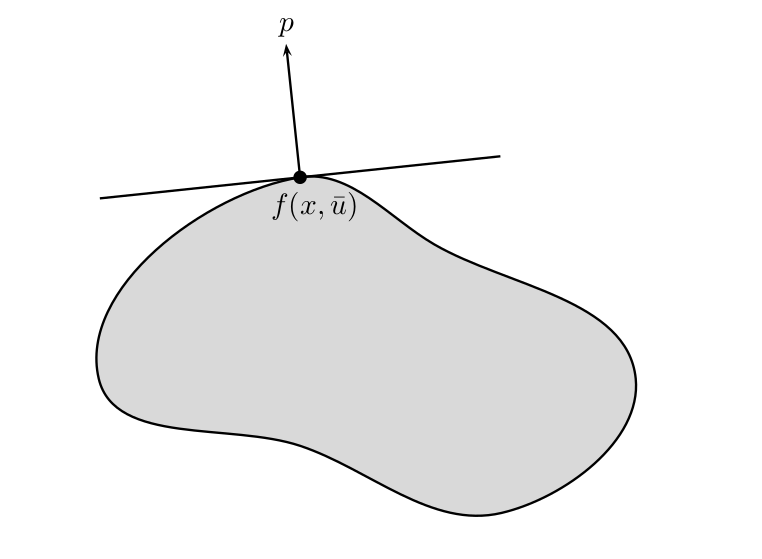
\includegraphics[width=\linewidth]{imgs/512-514.png}
	\caption{text}
	\label{fig-5.2}
\end{figure}

So now, 
\subparagraph[5.14]{Theorem:} Demonstration of theorem 5-14 is not that clear in the book, so for now, it is skipped.


\subsection{Controlled trajectories and boundary of reachable set}
The following very important theorem tell us two very important things. If, in the end (at $t_1$) the trajectory lies on the boundary of the reachable set, then first, there exists an adjoint response that maximizes the Hamiltonian for any instant in $\tzto$ (or, better to say, in the Lebesgue points for $f$ in that interval) and thus, secondly, the control is optimal, since it maximizes the Hamiltonian. \\
Formally said,

\subparagraph[5.16]{Theorem:} Given the usual control system, initial condition and time interval, given a control $\mu_*\in\admContr{\tzto}$, and given $\xi(\mu_*,x_0,t_0,t_1)$ (abbreviate $\xi(\mu_*,x_0,t_0,\cdot$ simply with $\xi_*$ ),\\
if $\xi_*(t_1) \in bd(\reachSetMath{t_1})$ then \lista{
	\item there exists an adjoint response $\lambda_*:\tzto\fd\R^n$ for $\Sigma$ for the controlled trajectory $(\xi_*,\mu_*)$, 
	\item $H_\Sigma(\xi(\mu_*,x_0,t_0,t),\lambda_*(t),\mu_*(t))=H_\Sigma^{max}(\xi(\mu_*,x_0,t_0,t),\lambda_*(t))$ for (almost) every $t\in\tzto$
}
\grass{Proof:} Since $\xi_*(t1)$ is on the boundary of the reachable set, then there exists a sequence $\{x_j\}$ in $\chi\backslash closure(\reachSetMath{t_1})$ that converges to that point. Now, let's take another sequence $v_j=\frac{x_j-\xi_*(t_1)}{||x_j-\xi_*(t_1)||}$. Since this sequence lies on the unitary sphere in $R^{n}$ and this set is compact, there exists a converging subsequence, that converges to $v_0$.\\
We now claim that $v_0\notin int(K(\mu_*,x_0,t_0,t_1))$:\\
\begin{minipage}{0.15\linewidth}
	 \mbox{}
\end{minipage}
\begin{minipage}{0.8\linewidth}
	 Supposing that $v_0$ lies in the internal part of the cone, then there exists a suffiecntly large $N$ such that, for $j>N$, every $v_j$ lies in the internal of the cone. Using the first theorem from the section "significative theorems" implies that for a certain $N$ also $x_{j>N}\in int(K(\mu_*,x_0,t_0,t_1))$. Indeed, a whole ball with center $\xi_*(t1)+v_j$ and radius $r$ is contained in the cone. In order to prove the last claim, the center of the ball is moved along the direction of $v_j$ until it coincides con $x_j$. One could (and should, in the case that $||x_j-\xi_*(t_1)||<1$) actually also re-scale the radius, and the re-scaled ball still lies in the cone. 
\end{minipage}\\
Given this, a topological lemma states that there exists a separating hyperplane $P(t_1)$ such that vector $v_0$ is contained in a half-space and the cone is contained in the other one.\\
Now take a the vector called $\lambda_*(t_1)$ orthogonal to $P(t_1)$ lying in the half space not containing the cone, and thus \[\langle \lambda_*(t_1),v\rangle\text{      }v\in K(\mu_*,x_0,t_0,t_1).\]
To conclude, we just need to take the unique adjoint response that has the value $\lambda_*(t_1)$ at time $t_1$, and use the preceding theorems. 

\paragraph{Interpretation}
In the following figures we can have a deeper insight of the passages and geometrical constructions behind this theorem. In the first figure, \ref{fig-5.3.1} one can see that the adjoint response points somehow "outside" of the reachable set. Indeed, if the objective is staying on the boundary of the expanding reachable set, it sounds logical to choose a control, and thus an $f(\xi,\mu)$ that "points outside the reachable set, as much as it can". This effort is represented in the maximization of the Hamiltonian,  which is, by the maximization of the scalar product between the possible $f$ and $\lambda$, as depicted in \ref{fig-5.2}. %\ref{fig-5.3.2}

\begin{figure}[h!]
	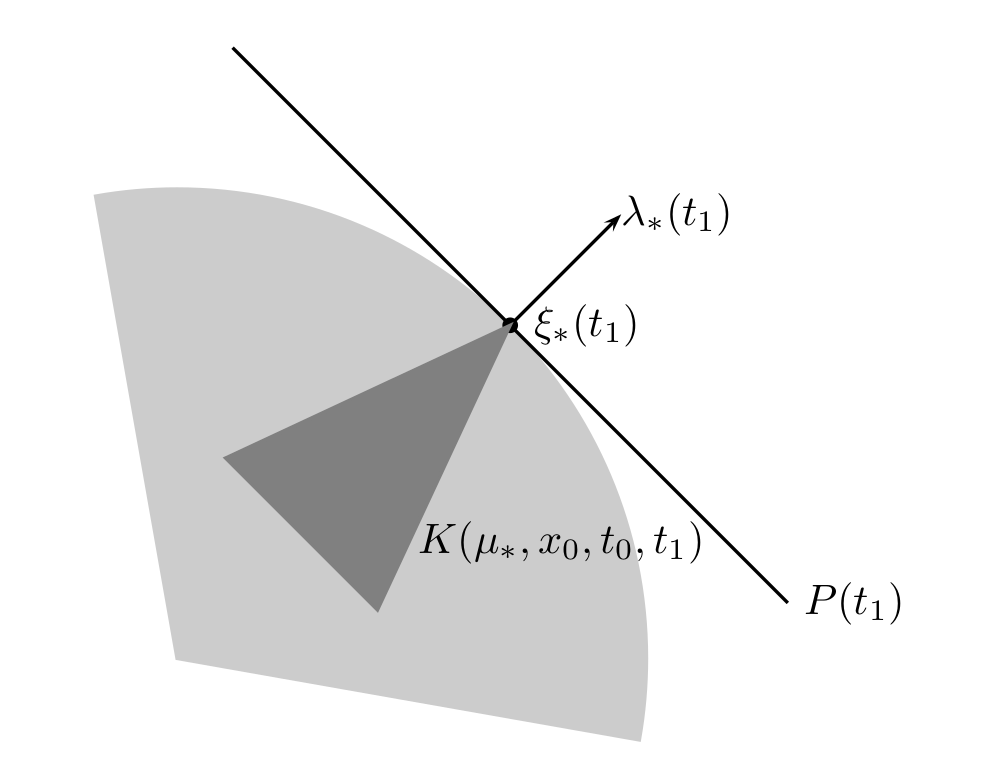
\includegraphics[width=0.4\linewidth]{imgs/5-3-L.png}
	\caption{"Zoom" on the cone, part of the reachable set and final point of the trajectory at the final instant}
	\label{fig-5.3.1}
\end{figure}

An important observation must be made, which is that the hyperplane actually separates the cone from the vector $v_0$ from the cone $K$, so the hyper plane does not have to be tangent to the reachable set, as seen in figure \grass{yet to draw the figure}. %\ref{fig-5.3.2}.\\
Finally, the last figure, shows us the evolution of the adjoint response, of the separating plane $P$ and of the trajectory (dotted in the figure). As already said, the control should be such that, instant by instant, the function steering the system $\statotdot$ has maximal projection in the direction of $\lambda$.
\begin{figure}[h!]
	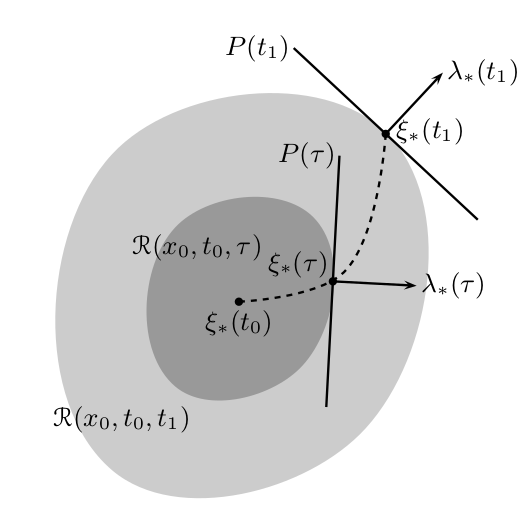
\includegraphics[width=\linewidth]{imgs/5-3-R.png}
	\caption{Depiction of the situation at two different instants, the final one and one intermediate, $\tau$}
\end{figure}
There is a last theorem for this section, which states that once a system is fallen from the border of the reachable set, it remains in its internal for all the successive instants. Basically, in a crowd of runners where everybody runs at the (same and uniform) maximum speed, once a runner diminishes the speed for an ammount of time that is not Lebesgue-neglettable, it will fall inside the crowd, and won't be able to return on the border anymore. 

\subparagraph[5.17]{Theorem:trajectories in the interior of the reachable set remain in the interior} Let's have the usual control system, initial condition, time interval and admissible control. If, for a certain instant $\tau\in[t_0,t_1)$ it happens that $\trajWinCondMath{\tau}\in int(\reachSetMath{\tau})$ then\\
\trajWinCond{t}$\in int(\reachSetMath{t})$ for all $t\in(\tau,t_1]$
\grass{TODO:PROOF. it requires to give as good that the map F is a diffeomorphism.}



\subsection{Extended system, extended reachable set and optimal trajectories}
Before stating the penultimate theorem, there is just another small definition to be made, which is the one of extended system, which is just the extension from n to n+1 dimensions for the state of the system, where the new, 0-th dimension is the value of the cost function so far.

\subparagraph[6.1]{Definition: Extended System} Let $L$ be a Lagrangian for control system \controlSystem. We define the \grass{extended system} as $\hat{\Sigma}=(\hat\chi,\hat{f},U)$ just by asking that \lista{
	\item $\hat\chi=\R\times\chi$
	\item $\hat f((x^0,x),u)=(L(x,u),f(x,u))$
}
Note that now the equations governing the extended system are 
\begin{gather*}
	 \dot{\xi}^0(t)=L(\statot,\mut)\\
	\statotdot=f(\statot,\mut)\\
	\implies\\
	\xi^0(\tau)=\int_{t_0}^{\tau}L(\statot,\mut)dt
\end{gather*}
Which is precisely the cost function.\\
There now will be an important theorem, that lies an important layer in the proof of the principle. In fact, so far, the optimality of a trajectory has always been related to the maximization of an Hamiltonian, as is stated in the proof of the principle. But, looking deeper into the previous theorems, the maximization of the Hamiltonian just ensures that the trajectory lies on the boundary of the reachable set (that it's always on the "frontline of runners, so to say". But the fact that the trajectory runs through the space of admissible states as possibile has nothing to do, a-priori, with the cost associated to that controlled trajectory. 
\subparagraph[6.2]{Theorem:}Let $L$ be a Lagrangian for control system \controlSystem, $\szm,\som\subset\chi$ be sets, and suppose that $(\xi_*,\mu_*)$ is a solution to the fixed interval problem (which is, $(\xi_*,\mu_*)\in\mathfrak{P}(\Sigma,L,\szm,\som,[t_0,t_1])$, then\\
$\hat{\xi}_*(t_1)\in boundary(\extReachSetStarMath{t_1})$\\
\grass{Proof:} Since $(\xi_*,\mu_*)\in\mathfrak{P}(\Sigma,L,\szm,\som,[t_0,t_1])$, then the corresponding extended trajectory has the obvious property that the cost $\xi^0(t_1)$ is the lowest possible among all the possible controlled arcs \controlledTraj that steer the system from $\xi_*(t_0)\text{ to }\xi_*(t_1)$. So given the set of "possible costs" , the first element of $\hat{\xi}_*(t_1)$ is obviously on the boundary of the said set (at least, as long as the trajectories are L-acceptable, which is, the integral represented by the cost function is finite). This must then imply that also $\hat{\xi}_*(t_1)$ is on the boundary of the extended reachable set: let's take a neighbourhood of $\hat{\xi}_*(t_1)$ in the extended state space $\hat{\chi}$. Any neighbourhood will then contain points of the form $(c,\xi_*(t_1))$ with $c<\xi_*^0(t_1)$. But those points, with a cost which is littler than the minimum one, are not in the extended reachable set by hypothesis, since the controlled trajectory  $(\xi_*,\mu_*)$ is optimal. So, since there is no neighbourhood of $\hat{\xi}_*(t_1)$ contained in \extReachSetStar{t_1}, th
is point must lie on the boundary, as wanted.\\\\


The fact that $\hat{\xi}_*(t_1)$ is on the boundary of the extended reachable set implies that the trajectory $\xi(t_1)$ is on the boundary of \reachSet{t_1}, thus implying the bond with cost-wise optimality and being on the boundary of the reachable set, which is an Hamiltonian-wise optimality. Indeed, it will be used in the following theorem.


\subsection[6.3]{Adjoint response, Hamiltonian and maximum principle}
Finally, we will now prove the points 1 to 3 in the statement of the principle. 

\subparagraph[6.3]{Theorem:}Let $L$ be a Lagrangian for control system \controlSystem, $\szm,\som\subset\chi$ be sets, and suppose that $(\xi_*,\mu_*)$ is a solution to the fixed interval problem (which is, $(\xi_*,\mu_*)\in\mathfrak{P}(\Sigma,L,\szm,\som,[t_0,t_1])$, then\\
There exists an absolutely continous map $\lambda_*:\tzto\fd\R^n$ and a number $\lambda_*^0\in\{-1,0\}$ with the following properties:
\begin{enumerate}
	\item either $\lambda_*^0=.1$ or $\lambda_*(t_0)\ne0$
	\item $\lambda_*$ is an adjoint repsonse for $(\Sigma,\lambda_*^0,L)\text{ along }(\xi_*,\mu_*)$
	\item $H_{\Sigma,\lambda_*^0L}(\xi_*(t),\lambda_*(t),\mu_*(t))=H_{\Sigma,\lambda_*^0L}^{max}(\xi_*(t),\lambda_*(t))$ for almost every $t\in[t_0,t_1]$
\end{enumerate}
\grass{Proof:} First, we observe that the vector $(-1,0_v)\in\R\times\R^n$ cannot lie in the interior of the extended tangent cone \extFixIntTanCone{t_1}. If this were not the case, by means of \label{REF REF REFERENCE TODO} the preceding theorems, there would be points $a^0,a$ in \extReachSetStar{t_1} at a lower cost, whose position in the state space is actually the same ($a=\xi_*(t_1)$). This would violate the optimality of $(\xi_*,\mu_*)$.\\
Since this vector does not lie in the internal of \extFixIntTanCone{t_1}, there exists a separating hyperplane $\hat P(t_1)$ between this cone and the vector. \\
Take a vector $\hat{\lambda}_*(t_1)$ orthogonal to $\hat P(t_1)$, in the half space not containing the cone. This implies 
\gatherNo{
	\langle \hat{\lambda}_*(t_1),(-1,0) \rangle\ge0;\\
	\langle \hat{\lambda}_*(t_1),\hat{v}\rangle\le0;\text{     }\hat{v}\in\extFixIntTanConeMath{t_1}
}
This implies then that $\hat{\lambda}_*^0(t_1)\leq0$.\\
Define then $\hat{\lambda}_*$ as the adjoint response whose value at $t_1$ is equal to $\hat{\lambda}_*(t_1)$.\\
From the equations for the adjoint response \ref{adjoint-equation} we obtain that $\dot{\lambda}_*^0(t)=0$. This is because since $\hat f$ does not depend on $x_0$, then the Jacobian matrix $\Dderarg{1}\hat f$ has the first column $0$, and thus the transposed matrix has the first row of zeros. This is of course by imagining the (extended) adjoint response as a coloumn vector.\\
So $\lambda_*^0(t)=0$ is constant and nonpositive. So, if $\lambda_*^0(t)\neq0$, we can rescale the whole extended adjoint response so that $\hat{\lambda}_*$ becomes $\frac{\hat{\lambda}_*}{-(\lambda_*^0)}$, so that now $\lambda_*^0$ is either 0 or -1.\\
Now, the Hamiltonian for the extended system is very similar to the extended Hamiltonian for the system (plus the Lagrangian):
\gatherNo{\hat{H}_{\hat{\Sigma}}\left((x^0,x),(p^0,p),u\right)=\langle p,f(x,u)\rangle+p^0L(x,u)=H_{\Sigma,p^0L}(x,p,u)}
Now, since the trajectory is optimal, by %REFERENCES 
\label{REFERENCES TO BE DONE!} virtue of the preceeding theorem, it lies on the boundary of the extended reachable se at time $t_1$. By means of the preceeding theorem %REFERENCES 
\label{REFREFREFREF3}
it holds that $H_{\Sigma,p^0L}(\xi_*(t),\lambda_*(t),\mu_*(t))=
H_{\Sigma,p^0L}^{max}(\xi_*(t),\lambda_*(t))$ for almost every $t\in\tzto$.\\
Actually, the last theorem used deals with the boundary of the reachable set and not extended system, but it is enough to imagine that the extended system is just a normal system with an added dimension. 